%%%%%%%%%%%%%%%%%
% (v1.1.5, 1 December 2018) written by LianTze Lim (liantze@gmail.com). Now compiles with pdfLaTeX, XeLaTeX and LuaLaTeX.
%
%% It may be distributed and
%%or modified under the
%% conditions of the LaTeX Project Public License, either version 1.3
%% of this license or (at your option) any later version.
%% The latest version of this license is in
%%    http://www.latex-project.org/lppl.txt
%% and version 1.3 or later is part of all distributions of LaTeX
%% version 2003/12/01 or later.
%%%%%%%%%%%%%%%%

%% If you need to pass whatever options to xcolor
\PassOptionsToPackage{dvipsnames}{xcolor}

%% If you are using \orcid or academicons
%% icons, make sure you have the academicons
%% option here, and compile with XeLaTeX
%% or LuaLaTeX.
% \documentclass[10pt,a4paper,academicons]{altacv}

%% Use the "normalphoto" option if you want a normal photo instead of cropped to a circle
% \documentclass[10pt,a4paper,normalphoto]{altacv}

\documentclass[10pt,a4paper,ragged2e]{altacv}

%% AltaCV uses the fontawesome and academicon fonts
%% and packages.
%% See http://texdoc.net/pkg/fontawesome and http://texdoc.net/pkg/academicons for full list of symbols. You MUST compile with XeLaTeX or LuaLaTeX if you want to use academicons.

% Change the page layout if you need to
\geometry{left=1.25cm,right=1.25cm,top=1.5cm,bottom=1.5cm,columnsep=1.2cm}

% The paracol package lets you typeset columns of text in parallel
\usepackage{paracol}

% Change the font if you want to, depending on whether
% you're using pdflatex or xelatex/lualatex
\ifxetexorluatex
  % If using xelatex or lualatex:
  \setmainfont{Lato}
\else
  % If using pdflatex:
  \usepackage[utf8]{inputenc}
  \usepackage[T1]{fontenc}
  \usepackage[default]{lato}
\usepackage{biblatex}
\fi

% Change the colours if you want to
\definecolor{Mulberry}{HTML}{72243D}
\definecolor{SlateGrey}{HTML}{2E2E2E}
\definecolor{LightGrey}{HTML}{666666}
\colorlet{heading}{Sepia}
\colorlet{accent}{Mulberry}
\colorlet{emphasis}{SlateGrey}
\colorlet{body}{LightGrey}

% Change the bullets for itemize and rating marker
% for \cvskill if you want to
\renewcommand{\itemmarker}{{\small\textbullet}}
\renewcommand{\ratingmarker}{\faCircle}
\linespread{0.9}
%% sample.bib contains your publications
\addbibresource{sample.bib}

\begin{document}
\name{\LARGE Cheat-Sheet: Datensicherung}
\tagline{\normalsize Der Begriff Datensicherung, auch als Backup bezeichnet, beschreibt das Kopieren von Daten, um diese im Falle eines Datenverlustes wiederherstellen zu können. Diese Wiederherstellung wird auch als Restore bezeichnet.}

  %% You MUST add the academicons option to \documentclass, then compile with LuaLaTeX or XeLaTeX, if you want to use \orcid or other academicons commands.
  % \orcid{orcid.org/0000-0000-0000-0000}

\makecvheader

%% Depending on your tastes, you may want to make fonts of itemize environments slightly smaller
% \AtBeginEnvironment{itemize}{\small}

%% Set the left/right column width ratio to 6:4.
\columnratio{0.5}

% Start a 2-column paracol. Both the left and right columns will automatically
% break across pages if things get too long.
\begin{paracol}{2}
\cvsection{\Large Arten}

\begin{itemize}
\item \textbf{\Large Vollsicherung}
\vspace{3mm}
    \newline Vollständige Sicherung aller Daten.
    \vspace{3mm}
    \begin{itemize}
        \item \large Vorteile:
        \vspace{1mm}
            \newline \textendash \normalsize Einfache Wiederherstellung für die nur ein Medium benötigt wird.
        \vspace{3mm}
        \item \large Nachteile:
        \vspace{1mm}
             \newline \textendash \normalsize Sehr hoher Speicherbedarf.
             \vspace{1mm}
             \newline\textendash \normalsize Für mehrere Versionen müssen mehrere Medien aufbewahrt werden
        
    \end{itemize}
    
    \begin{center}
        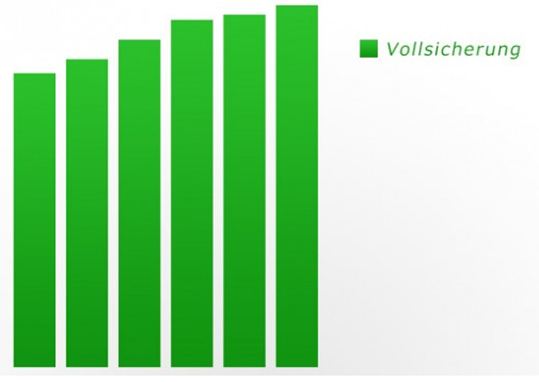
\includegraphics[width=0.35\textwidth]{full.png}
    \end{center}
    
    \divider
\item \textbf{\Large Differentielle Sicherung}
\vspace{3mm}
\newline Sicherung aller Daten, die seit der letzten Vollsicherung verändert wurden.
\vspace{3mm}
    \begin{itemize}
        \item \large Vorteile:
        \vspace{1mm}
            \newline \textendash \normalsize Weniger Speicherbedarf als der Vollsicherung
        \vspace{3mm}
        \item \large Nachteile:
        \vspace{1mm}
             \newline \textendash \normalsize Die Wiederherstellung ist langsamer, da i.d.R. zwei Medien benötigt werden. (Letzte Vollsicherung und letzte differentielle Sicherung)
        
    \end{itemize}
    \begin{center}
        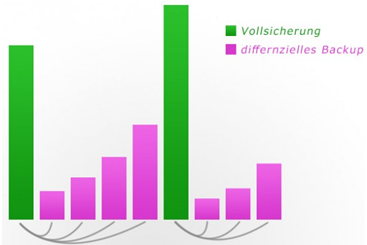
\includegraphics[width=0.35\textwidth]{differential.png}
    \end{center}
\divider
\begin{thebibliography}{9}

\bibitem{typeReference} 
Sicherungsstrategien,
\\\texttt{Informationsmaterial ITECH}

\end{thebibliography}

\switchcolumn

\item \textbf{\Large Inkrementelle Sicherung}
\vspace{3mm}
\newline Sicherung der Daten, sie seit der letzten Sicherung (inkrementell, differentiell oder vollständig) verändert wurden.
\vspace{3mm}
    \begin{itemize}
        \item \large Vorteile:
        \vspace{1mm}
            \newline\textendash \normalsize Niedriger Speicherbedarf (aufgrund kleinerer inkrementeller Backups) 
        \vspace{3mm}
        \item \large Nachteile:
        \vspace{1mm}
    \newline\textendash \normalsize Zur Wiederherstellung sind das Vollbackup und alle seitdem erstellten inkrementellen Backups notwendig
    Wiederherstellung ist durch die Anzahl der benötigten Medien langsamer 
    \end{itemize}
\end{itemize}

\begin{center}
    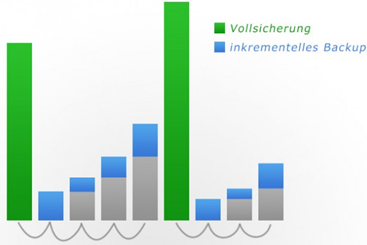
\includegraphics[width=0.35 \textwidth]{increment.png}
\end{center}

\cvsection{\Large Sicherungsstrategien}

\cvachievement{\LARGE\faHddO}{\Large First In, First Out (FIFO)}{
    \begin{itemize}
        \item Einfachste Strategie
        \item Backups werden auf den vorhandenen Medien gespeichert
        \item Wenn alle Medien belegt sind, werden die Daten des ältesten Mediums gelöscht
    \end{itemize}
}
\cvachievement{\LARGE\faRefresh}{\Large Generationenprinzip/ \newline Großvater-Vater-Sohn-Prinzip}{
    \begin{itemize}
        \item Großvater: Monatliche Vollsicherung mit jährlichem Rotationszyklus
        \item Vater: Wöchentliche Vollsicherung mit monatlichen Rotationszyklus
        \item Sohn: Tägliche differenzielle oder inkrementelle Sicherung mit wöchentlichem Rotationszyklus
    \end{itemize}
}
\cvachievement{\LARGE\faTasks}{\Large Türme von Hanoi}{
    \begin{itemize}
        \item Name geht auf das gleichnamige Spiel zurück
        \item Häufigkeit der Verwendung der Medien:
            \begin{itemize}
                \item Medium A: Jeder 2. Tag
                \item Medium B: Jeder 4. Tag
                \item Medium C: Jeder 8. Tag
                \item Medium n: Jeder 2n. Tag
            \end{itemize}
    \end{itemize}
}

\end{paracol}

\end{document}
